\begin{wrapfigure}[0]{r}[-2.5cm]{3cm}
 \vspace{-6cm}
 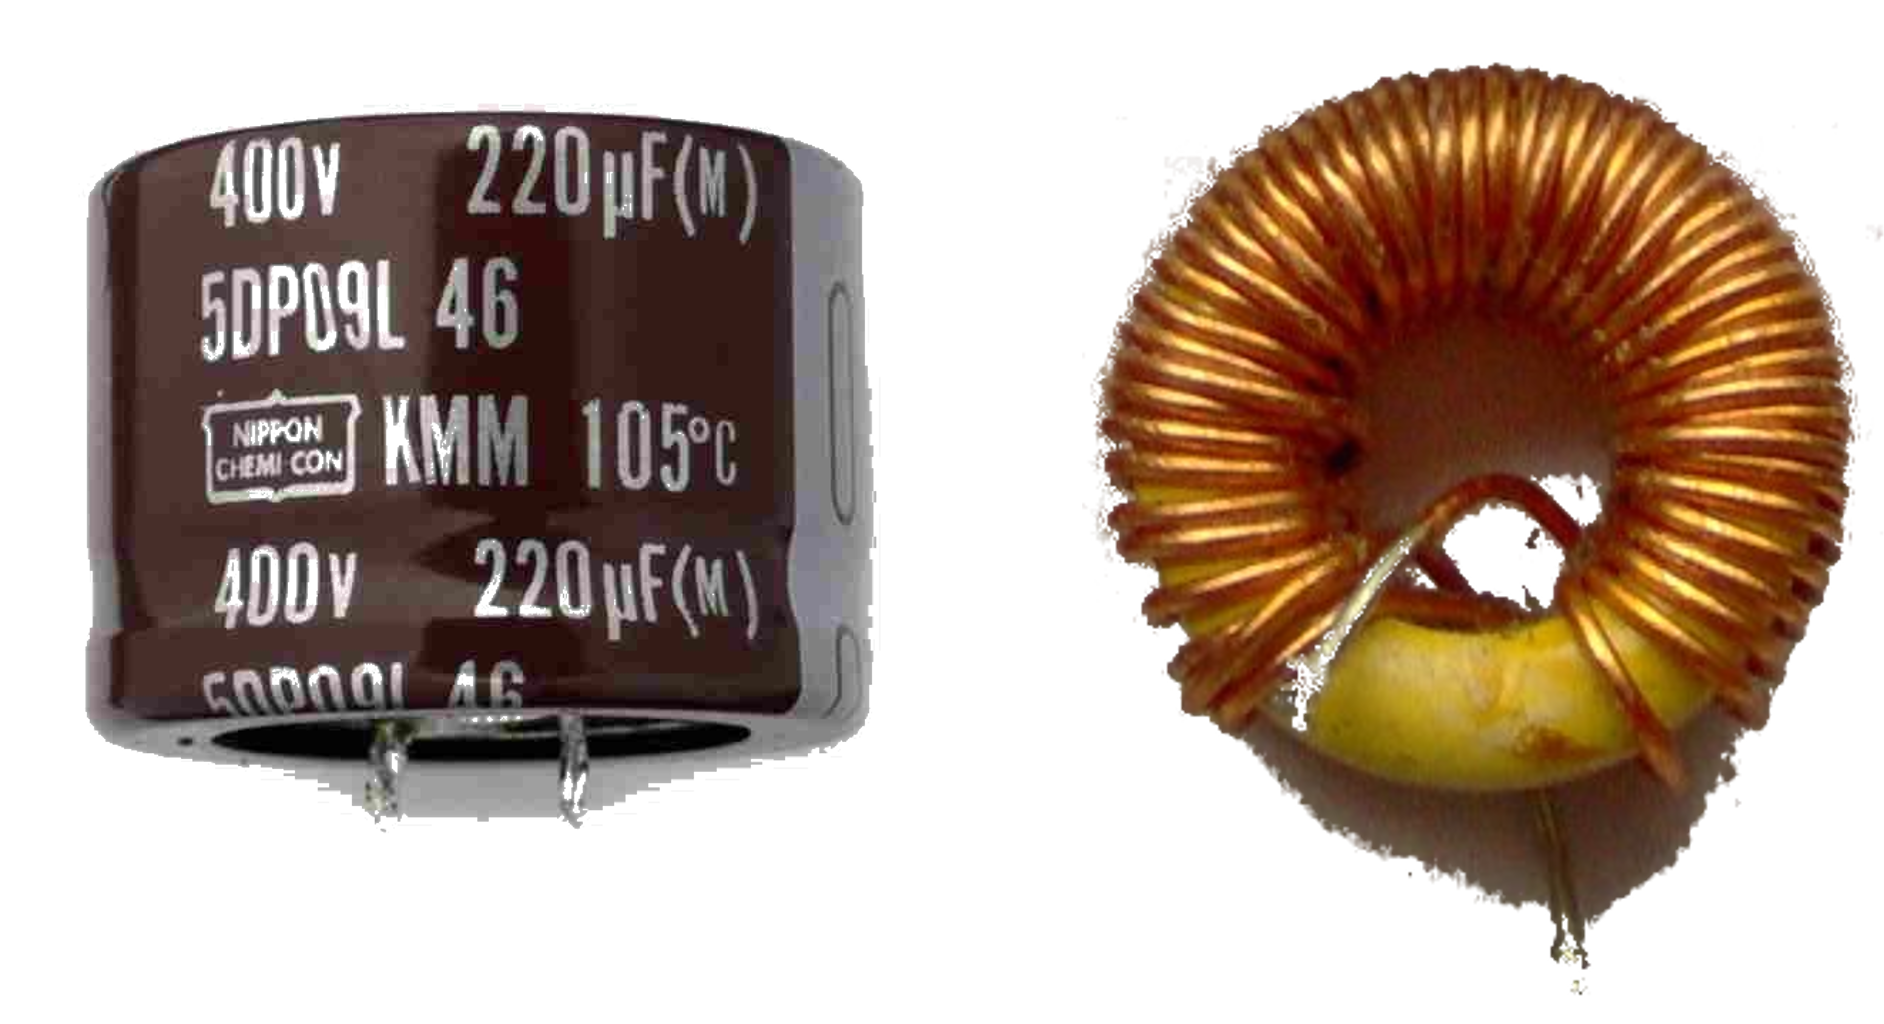
\includegraphics[scale=0.4]{KondensatorSpule/Bilder/KondensatorSpule.png}
 \vspace{-6cm}
\end{wrapfigure}

\section*{Theorie- und Prüfungsfragen} 


\mucho{1}{TC204}
{Wie verhält sich der Wechselstromwiderstand eines Kondensators mit zunehmender Frequenz?}%Frage
{Er bleibt konstant.}%A
{Er nimmt zu.}%B
{Er nimmt ab.}%C
{Er wird unendlich.}%D
{C}%Lösung

\mucho{2}{TC205}
{Wie groß ist der kapazitive Widerstand eines 10-pF-Kondensators bei 100 MHz?}%Frage
{31,8 $\Omega$}%A
{159 $\Omega$}%B
{318 $\Omega$}%C
{1,58 $k\Omega$}%D
{B}%Lösung

\mucho{3}{TC203}
{Ein verlustloser Kondensator wird an eine Wechselspannungsquelle angeschlossen. Welche Phasenverschiebung zwischen Spannung und Strom stellt sich ein?}%Frage
{Die Spannung eilt dem Strom um 45$^\circ$ voraus.}%A
{Der Strom eilt der Spannung um 45$^\circ$ voraus.}%B
{Der Strom eilt der Spannung um 90$^\circ$ voraus.}%C
{Die Spannung eilt dem Strom um 90$^\circ$ voraus.
}%D
{C}%Lösung

\mucho{4}{TC207}
{Was versteht man unter dem Blindwiderstand eines Kondensators und von welchen physikalischen Größen hängt er ab?}%Frage
{Der Blindwiderstand ist der Wechselstromwiderstand eines Kondensators. Er ist abhängig von der Kapazität des Kondensators und der anliegenden Frequenz. Im Blindwiderstand entstehen keine Wärmeverluste.}%A
{Der Blindwiderstand ist der Gleichstromwiderstand eines Kondensators. Er ist abhängig vom Isolationsmaterial des Kondensators und der anliegenden Spannung. Auch im Blindwiderstand entstehen Wärmeverluste.}%B
{Der Blindwiderstand ist der Wechselstromwiderstand eines Kondensators. Er ist abhängig von der Blindkapazität des Kondensators und der anliegenden Spannung. Im Blindwiderstand entstehen hohe Verluste.}%C
{Der Blindwiderstand ist der HF-Gleichstromwiderstand eines Kondensators. Er wird mit steigender Kapazität sowie bei erhöhtem Wechselstromanteil und steigender Frequenz größer. Je höher die Frequenz umso eher wandern die Ladungen an die Plattenränder (Skin-Effekt).}%D
{A}%Lösung

\mucho{5}{TD103}
{Wie groß ist die Gesamtkapazität von drei parallel geschalteten Kondensatoren von 20$nF$, 0,03$\mu F$ und 15000$pF$?}%Frage
{0,650$\mu F$}%A
{650$nF$}%B
{0,065$\mu F$}%C
{650000 $pF$
}%D
{C}%Lösung

\mucho{6}{TC310}
{Mit einem Schalenkern, dessen AL-Wert mit 250 angegeben ist, soll eine Spule mit einer Induktivität von 2$mH$ hergestellt werden. Wie groß ist die erforderliche Windungszahl?}%Frage
{3}%A
{53}%B
{89}%C
{2828}%D
{C}%Lösung


\mucho{7}{TC306}
{Was versteht man unter dem Blindwiderstand einer Spule und von welchen physikalischen Größen hängt er ab?}%Frage
{Der Blindwiderstand ist der Wechselstromwiderstand einer Spule. Er ist abhängig von der Induktivität der Spule und der anliegenden Frequenz. Im Blindwiderstand entstehen keine Wärmeverluste.}%A
{Der Blindwiderstand ist der Gleichstromwiderstand einer Spule. Er ist abhängig vom Isolationsmaterial der Spule und der anliegenden Spannung. Auch im Blindwiderstand entstehen Wärmeverluste.}%B
{Der Blindwiderstand ist der Wechselstromwiderstand einer Spule. Er ist abhängig von der Blindinduktivität der Spule und der anliegenden Spannung. Im Blindwiderstand entstehen hohe Verluste.}%C
{Der Blindwiderstand ist der HF-Gleichstromwiderstand einer Spule. Er wird mit steigender Induktivität sowie bei erhöhtem Wechselstromanteil und steigender Frequenz größer. Je tiefer die Frequenz umso eher wandern die Elektronen an den Spulenrand (Skin-Effekt).}%D
{A}%Lösung

\mucho{6}{TC305}
{Wie groß ist der Wechselstromwiderstand einer Spule mit 3$\mu H$ Induktivität bei einer Frequenz von 100 MHz?}%Frage
{1,9$\Omega$}%A
{942$\Omega$}%B
{1885$\Omega$}%C
{1885$k\Omega$}%D
{C}%Lösung

\mucho{6}{TC302}
{In einer reinen Induktivität, die an einer Wechselspannungsquelle angeschlossen ist, eilt der Strom der angelegten Spannung ...}%Frage
{um 90 $^\circ$ voraus.}%A
{um 90 $^\circ$ nach.}%B
{um 45 $^\circ$ voraus.}%C
{um 45 $^\circ$ nach.}%D
{B}%Lösung